\chapter{Ulepszenia}

W poprzednich rozdziałach przedstawiono wyniki algorytmu kodującego. Ponieważ nie są one zadowalające pomyślano nad sposobom poprawy algorytmu. Wadliwe działanie można usprawiedliwiać zbyt trudnym dopasowaniem kodów, ponieważ nie uwzględniano sąsiednich kratek kodowych. Podjęto więc decyzję o zmianie algorytmu w taki sposób aby porównywać nie tylko bezpośrednio odpowiadające kratki kodu, ale również ich sąsiadów. Tak więc dopasowanie jest nie tylko gdy zgodne są wszystkie współrzędne kodu x, y i kąt, ale również dopasowanie gdzie dowolna ze współrzędnych jest przesunięta o 1 kratkę kodową w górę lub w dól. Rozwiązanie sprzyja dopasowaniu kodów i powinno w jakiś sposób rekompensować nieliniowe przekształcenia opuszka palca. 
\begin{figure}[!htb]
    \begin{center}
		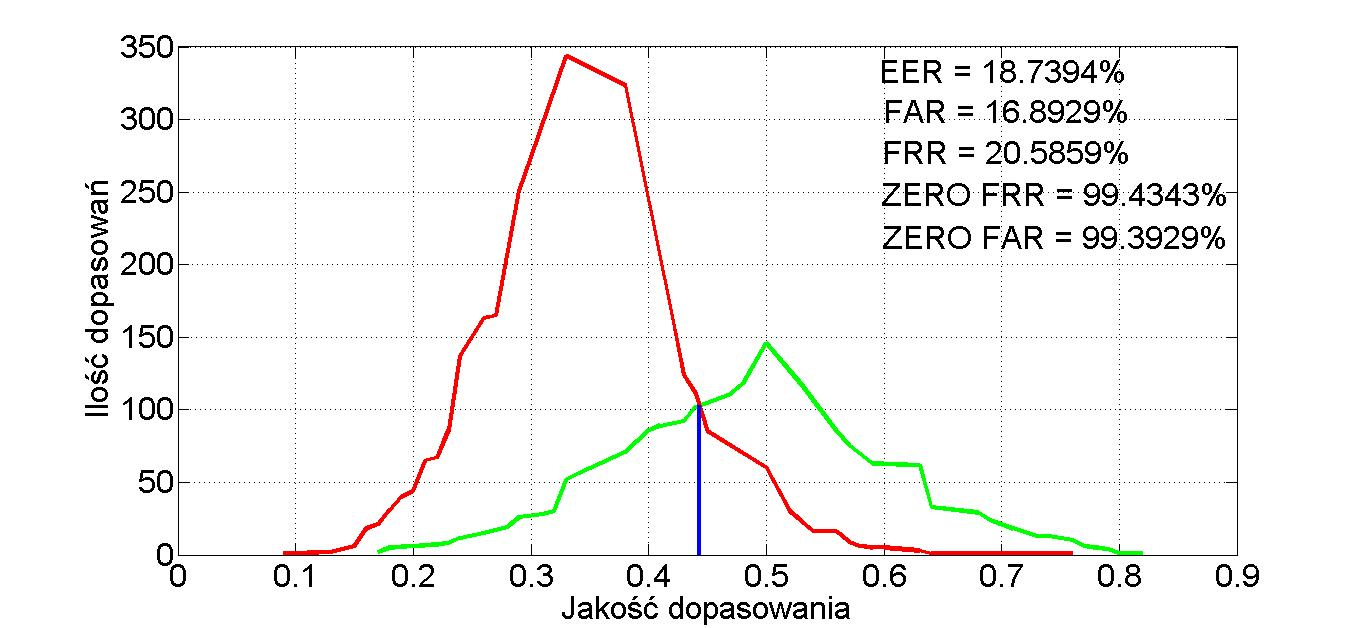
\includegraphics[angle=0,scale=0.35]{img/pattern_line_statistic_better_code.jpg}
		\caption{Ilość dopasowań w zależności od jakości dopasowania do odcisku wzorca (poprawiony algorytm)}
		\label{img:pattern_better_code}
    \end{center}
\end{figure} 

Wykresy \ref{img:pattern_better_code} oraz \ref{img:sample_better_code} prezentują wyniki poprawionego algorytmu. Wskaźnik EER poprawił się tylko nieznacznie z 17\%-21\% na 18\% - 19\%. FAR zmienił się z 11\% - 25\% na 13\% - 16\%. FRR z 17\% - 23\% na 21\% - 20\%. Jednak ogólna ocena mówi o niewielkiej zmianie przedstawionej modyfikacji algorytmu.

\begin{figure}[!htb]
    \begin{center}
		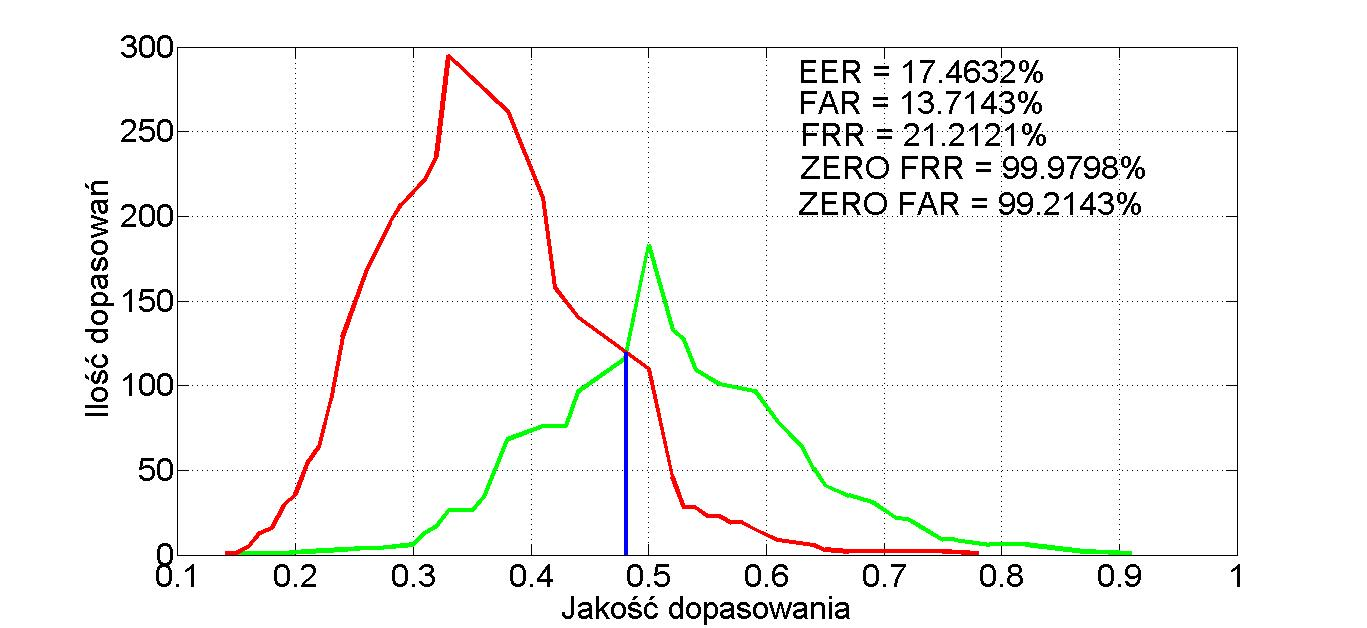
\includegraphics[angle=0,scale=0.35]{img/sample_line_statistic_better_code.jpg}
		\caption{Ilość dopasowań w zależności od jakości dopasowania do odcisku próbki (poprawiony algorytm)}
		\label{img:sample_better_code}
    \end{center}
\end{figure} 

Natomiast dal analizy różnicy symetrycznej wyniki nieco się poprawiły. EER spadł z 16\% na 13\%, FAR wzrósł z 12\% na 14\%, a FRR spadł z 17\% na 13\%. Wyniki przedstawione są na wykresie \ref{img:simetric_better_code}
\begin{figure}[!htb]
    \begin{center}
		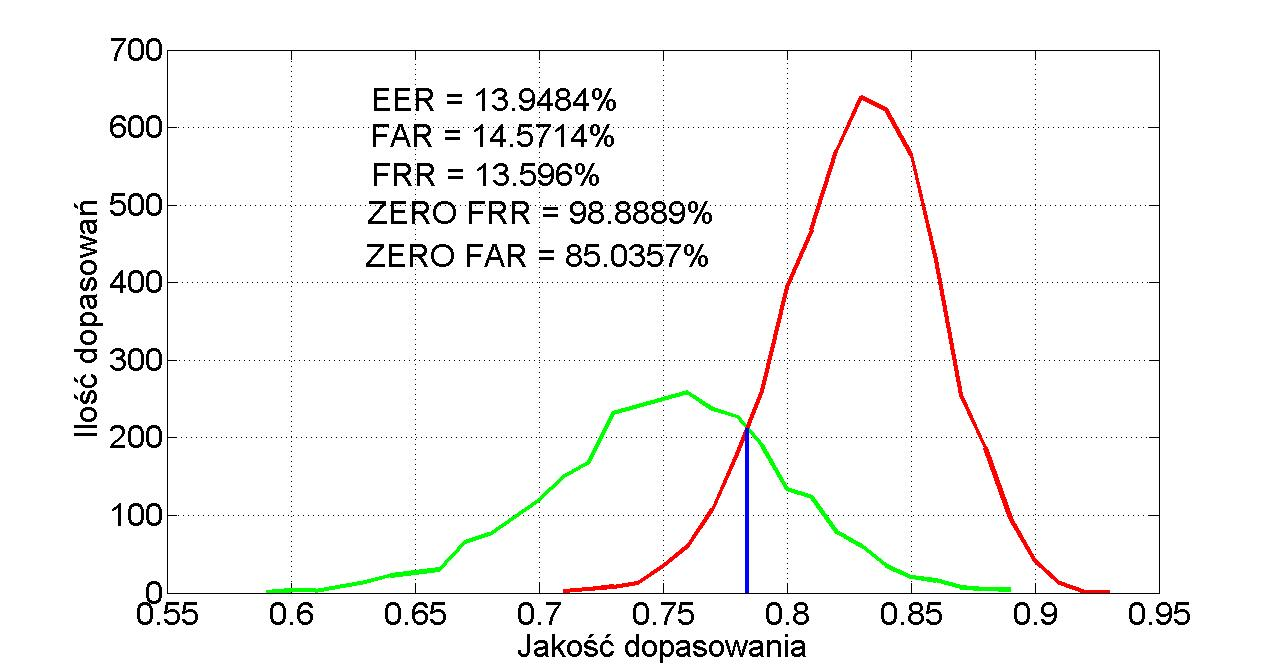
\includegraphics[angle=0,scale=0.4]{img/simetric_distance_better_code_line.jpg}
		\caption{Ilość niedopasowań w zależności od jakości niedopasowania do odcisków}
		\label{img:simetric_better_code}
    \end{center}
\end{figure} 

Tabele \ref{tab:3D_sum_21}, \ref{tab:3D_sum_22} i \ref{tab:3D_sum_23} przedstawiają wyniki metody 3D. Porównywania kodów również uzyskały podobne wyniki jak w niepoprawianej wersji algorytmu. Biorąc pod uwagę najlepszy wynik metod poprawiła się o ok 4 punkty procentowe. Globalnie metoda 3D tak jak i poprzednio wypadła znacznie gorzej niż analizowanie różnicy symetrycznej. Identycznie jak w poprzednich przypadkach przyczyną jest niemożliwość separowania zbiorów punktów porównań. 

\begin{table}[!htb]
    \begin{tabular}{p{3cm}|r||c|c|c|}
	\cline{2-5}
    & Wariant & \multicolumn{3}{|c|}{1:1 do 1:0 + 0:1}\\ \cline{2-5} 
    & Zbiór testujący & ERRORS  & FRR & FAR\\ \hline
	\multicolumn{2}{|l||}{Rodzaj jądra} &  \multicolumn{3}{|c|}{}\\
	\hline\hline
    \multicolumn{2}{|l||}{Liniowe} & 25.7359\% & 27.9635\% & 22.9755\%\\ \hline
    \multicolumn{2}{|l||}{Kwadratowe} & 26.1564\% & 31.1550\% & 19.9623\%\\ \hline
    \multicolumn{2}{|l||}{Wielomianowe st. 3} & 25.9882\% & 30.2432\% & 20.7156\%\\ \hline
    \multicolumn{2}{|l||}{Wielomianowe st. 7} & 29.5206\% & 31.6109\% & 26.9303\%\\ \hline
    \multicolumn{2}{|l||}{Wielomianowe st. 12} & 30.6981\% & 29.9392\% & 31.6384\%\\ \hline
    \multicolumn{2}{|l||}{Normalne(Gaussowskie)} & 26.0723\% & 33.2827\% & 17.1375\%\\ \hline
    \end{tabular}
	\caption{Wyniki testów poprawionego algorytmu kodowego metoda 3D porównywania kodów}
	\label{tab:3D_sum_21}
\end{table}

\begin{table}[!htb]
    \begin{tabular}{p{3cm}|r||c|c|c|}
	\cline{2-5}
    & Wariant & \multicolumn{3}{|c|}{1:1 do 1:0}\\ \cline{2-5} 
    & Zbiór testujący & ERRORS  & FRR & FAR\\ \hline
	\multicolumn{2}{|l||}{Rodzaj jądra} &  \multicolumn{3}{|c|}{}\\
	\hline\hline
    \multicolumn{2}{|l||}{Liniowe} & 31.2500\% & 19.0283\% & 48.3051\%\\ \hline
    \multicolumn{2}{|l||}{Kwadratowe} & 32.6651\% & 16.3968\% & 55.3672\%\\ \hline
    \multicolumn{2}{|l||}{Wielomianowe st. 3} & 31.8396\% & 17.4089\% & 51.9774\%\\ \hline
    \multicolumn{2}{|l||}{Wielomianowe st. 7} & 34.7877\% & 16.5992\% & 60.1695\%\\ \hline
    \multicolumn{2}{|l||}{Wielomianowe st. 12} & 35.6132\% & 15.9919\% & 62.9944\%\\ \hline
    \multicolumn{2}{|l||}{Normalne(Gaussowskie)} & 34.9057\% & 4.0486\% & 77.9661\%\\ \hline
    \end{tabular}
	\caption{Wyniki testów poprawionego algorytmu kodowego metoda 3D porównywania kodów}
	\label{tab:3D_sum_22}
\end{table}

\begin{table}[!htb]
    \begin{tabular}{p{3cm}|r||c|c|c|}
	\cline{2-5}
    & Wariant & \multicolumn{3}{|c|}{1:1 do 0:1}\\ \cline{2-5} 
    & Zbiór testujący & ERRORS  & FRR & FAR\\ \hline
	\multicolumn{2}{|l||}{Rodzaj jądra} &  \multicolumn{3}{|c|}{}\\
	\hline\hline
    \multicolumn{2}{|l||}{Liniowe} & 29.4652\% & 28.4872\% & 30.4979\%\\ \hline
    \multicolumn{2}{|l||}{Kwadratowe} & 30.5752\% & 34.5776\% & 26.3485\%\\ \hline
    \multicolumn{2}{|l||}{Wielomianowe st. 3} & 30.4743\% & 33.2024\% & 27.5934\%\\ \hline
    \multicolumn{2}{|l||}{Wielomianowe st. 7} & 30.4743\% & 32.6130\% & 28.2158\%\\ \hline
    \multicolumn{2}{|l||}{Wielomianowe st. 12} & 31.7861\% & 33.0059\% & 30.4979\%\\ \hline
    \multicolumn{2}{|l||}{Normalne(Gaussowskie)} & 29.9697\% & 34.9705\% & 24.6888\%\\ \hline
    \end{tabular}
	\caption{Wyniki testów poprawionego algorytmu kodowego metoda 3D porównywania kodów}
	\label{tab:3D_sum_23}
\end{table}


\vspace{5cm}\par
\section{Wnioski}
Oceniając zastosowane ulepszenie należy odnieść się do najlepszego uzyskanego wyniku, czyli analizy różnicy symetrycznej. Pomimo iż wskaźniki uległy poprawie nie należy uzyskanego wyniku uważać za satysfakcjonujący. 13\% wynik nie jest akceptowalny dla systemów biometrycznych. Dodatkowo próby uzyskania błędów zerowych kończą się podobnie jak w niepoprawianej wersji algorytmu. Dla takich progów błędy FAR i FRR wynoszą ponad 80\%. Świadczy to o wysokiej nieprzydatności zastosowanego rozwiązania. Pod sporym znakiem zapytania stoi również możliwość stosowania metod kodowania odcisku. Najważniejszym problemem jest niemożliwość spojrzenia na wszystkie minucje naraz. Oznacza to, że za każdym razem algorytm kodowania porównuje ze sobą dwa pojedyncze punkty i nie wie czy porównanie to ma jakikolwiek sens. Algorytmy obiektowe reprezentują minucje jako obiekty w programie, łatwe jest spojrzenie globalne na odcisk i wykluczanie dopasowań niemożliwych. Dla algorytmu kodującego porównanie kodu jest binarne i widzi on tylko pojedyncze elementy kodu.